\documentclass{scrartcl}

\usepackage{Header}

\usepackage{hyperref} %for links
%\usepackage{algorithmic} %for pseudocode

\begin{document}


\Gruppe{Stephan Heidinger}{AlgoDat - Zusammenfassung v0.1}
\Header{Algorithemn \& Datenstrukturen}{Wintersemester 2011/2012}{Stephan Heidinger}{}%leave last variable empty, else there will be aufgabenblatt überschrift

\begin{shaded}
Dieses Dokument wurde unter der Creative Commons - Namensnennung-NichtKommerziell-Weitergabe unter gleichen Bedingungen (\textbf{CC by-nc-sa}) veröffentlicht. Die Bedingungen finden sich unter \href{http://creativecommons.org/licenses/by-nc-sa/3.0/de}{diesem Link}. \\
\centerline{
\includegraphics[scale=1]{../cc-by-nc-sa.png} }
\end{shaded}

\textit{Find any errors? Please send them back, I want to keep them!}

\section{Einführung}
\subsection{Auswahlproblem}
Ziel: "`Bestimme das $k$. kleinste Element von $n$ Elementen"' \\
Spezialfälle: $k=
\begin{cases}
1 & Minimumsuche \\
n & Maximumsuche \\
\lfloor \frac{n}{2} \rfloor & Median
\end{cases}$\\

Verschiedene Ansätze:
\begin{enumerate}
	\item Auswahl nach Sortieren
	\item Wiederholte Minimumsuche
	\item Aktualisierung einer vorläufigen Lösung
	\item Nutzen von Standartbibliotheken
\end{enumerate}
Bewertung ist schwer, bei $1$ und $4$ muss mehr über die Implementierung bekannt sein, bei allen Varianten muss zudem mehr über die Eingabe bekannt sein.

\subsection{Maschinenmodell}
Wie soll bewertet werden? Laufzeit in Sekunden? Hängt massgeblich ab von:
\begin{itemize}
	\item Programmiersprache
	\item Rechner (Aufbau, Taktfrequenz, Speicher, \dots)
	\item Eingabedaten
\end{itemize}

Müssen Bewertung unabhängig davon finden $\Rightarrow$ \textbf{Zählen von \emph{elementaren Schritten}}

\begin{shaded}
\textbf{Random Access Machine} \\

Maschinenmodell mit:

\begin{itemize}
	\item endliche Zahl an Speicherzellen für Programm
	\item abzählbar endliche Zahl von Speicherzellen für Daten
	\item endliche Zahl von Registern
	\item arithmetisch-logische Einheit (ALU)
\end{itemize}

Anweisungen:

\begin{itemize}
	\item Transportbefehle (Laden, Verschieben, Speichern)
	\item Sprungbefehle (bedingt, unbedingt; $\to$ Schleifen, Rekursionen)
	\item arithmetische und logische Vernküpfungen
\end{itemize}

\end{shaded}

\subsection{Komplexität}
Beschreiben Komplexität durch.
\begin{description}
	\item[Laufzeit:] Anahl Schritte (asymptotisch)
	\item[Speicherbedarf:] Anzahl benutzter Speicherzellen
\end{description}

\subsubsection{Definitionen}
\begin{enumerate}
	\item höchstens so schnell wachsen wie $f$, {\tiny langsamer und gleich als $f$}
	\begin{shaded}
	\[ \mathcal{O}(f(n)) = \left\lbrace g: \mathds{N}_0 \to \mathds{R}
	\begin{array}{c}
	\textrm{es gibt Konstanten } c,n_0>0 \textrm{ mit} \\
	\vert g(n) \vert \leq c \cdot \vert f(n) \vert \textrm{ für alle } n>n_0
	\end{array}
	\right\rbrace \]
	\end{shaded}
	\item mindestens so schnell wachsen wie $f$, {\tiny schneller und gleich als $f$}
	\begin{shaded}
	\[ \Omega (f(n)) = \left\lbrace g: \mathds{N}_0 \to \mathds{R}
	\begin{array}{c}
	\textrm{es gibt Konstanten } c,n_0>0 \textrm{ mit} \\
	c \cdot \vert g(n) \vert \geq \vert f(n) \vert \textrm{ für alle } n>n_0
	\end{array}
	\right\rbrace \]
	\end{shaded}
	\item genauso so schnell wachsen wie $f$
	\begin{shaded}
	\[ \Theta(f(n)) = \left\lbrace g: \mathds{N}_0 \to \mathds{R}
	\begin{array}{c}
	\textrm{es gibt Konstanten } c_1,c_2,n_0>0 \textrm{ mit} \\
	c_1 \leq \frac{\vert g(n) \vert}{\vert f(n) \vert} \leq c_2 \textrm{ für alle } n>n_0
	\end{array}
	\right\rbrace \]
	\end{shaded}
	\item die gegenüber $f$ verschwinden, {\tiny langsamer als $f$}
	\begin{shaded}
	\[ o(f(n)) = \left\lbrace g: \mathds{N}_0 \to \mathds{R}
	\begin{array}{c}
	\textrm{zu jedem } c>0 \textrm{ex. \emph{ein} } n_0>0 \textrm{ mit} \\
	c \cdot \vert g(n) \leq \vert f(n) \vert \textrm{ für alle } n>n_0
	\end{array}
	\right\rbrace \]
	\end{shaded}
	\item denen gegenüber $f$ verschwindet, {\tiny schneller als $f$}
	\begin{shaded}
	\[ \omega(f(n)) = \left\lbrace g: \mathds{N}_0 \to \mathds{R}
	\begin{array}{c}
	\textrm{zu jedem } c>0 \textrm{ex. \emph{ein} } n_0>0 \textrm{ mit} \\
	\vert g(n) \geq c \cdot \vert f(n) \vert \textrm{ für alle } n>n_0
	\end{array}
	\right\rbrace \]
	\end{shaded}
\end{enumerate}

\begin{shaded}
\[ \log_a{n} \leq \sqrt{n} \leq n^2 \leq n^3 \leq 1,1^n \leq 2^n \leq n! \leq n^n\]
\end{shaded}

\subsubsection{Satz}
\begin{enumerate}
	\item $g \in \mathcal{O}(f) $ genau dann, wenn $f \in \Omega(g) $
	\\ $g \in \Theta(f) $ genau dann, wenn $f \in \Theta(g) $
	\item $\log_b{n} \in \Theta (\log_2{n}) $ für alle $b>1$ \\
	"`Die Basis des Logarithmus spielt für das Wachstum keine Rolle"'
	\item $ (\log_2{n})^d \in o(n^\varepsilon) $ für alle $d \in \mathds{N}_0, \varepsilon>0$\\
	"`Logarithmen wachsen langsamer als alle Polynomialfunktionen "'
	\item $ n^d \in o((1+\varepsilon)^n) $ für alle $d\in \mathds{N}_0, \varepsilon>0$\\
	"` Exponentielles Wachstum ist immer schneller als polynomielles "'
	\item $ b^n \in o((b+\varepsilon)^n) $ für alle $b\geq 1, \varepsilon>0$ \\
	"` Jede Verringerung der Basis verlangt exponentielles Wachstum"'
	\item $ \binom{a}{b} \in \Theta(n^k)$
	\item $H_n := \sum^n_{k=1} \frac{1}{k} = \ln n + \mathcal{O}(1)$ {\tiny (harmonische Zahlen)}
	\item $n! = \sqrt{2\pi n} \cdot \left( \frac{n}{c}^n \right) \cdot \left( 1+\Theta \left( \frac{1}{n} \right) \right)$ {\tiny (Stirlingformel)}
\end{enumerate}

%%%%%%%%%%%%%%%%%%%%%%%%%%%%%%%%%%%%%%%%%%%%%%%%%%%%%%%%%%%%%%%%%%%%%%%%%%%%%%%%%%%%%%%%
%%%%%%%%%%%%%%%%%%%%%%%%%%%%%%%%%%%%%%%%%%%%%%%%%%%%%%%%%%%%%%%%%%%%%%%%%%%%%%%%%%%%%%%%
%%%%%%%%%%%%%%%%%%%%%%%%%%%%%%%%%%%%%%%%%%%%%%%%%%%%%%%%%%%%%%%%%%%%%%%%%%%%%%%%%%%%%%%%


\section{Sortieren}
\subsubsection{Gütekriterien}
\begin{itemize}
	\item Laufzeit
	\item Speicherbedarf
	\item Stabilität (kein Vertauschen der Reihenfolge schon sortierter Elemente)
	\item u.U. getrennte Betrachtung von Anzahl Vergleiche $C(n)$ und Anzahl Umspeicherungen $M(n)$
\end{itemize}

\subsection{SelectionSort}
\subsubsection{Algorithmus}
Idee: Man nehme pro Durchlauf das kleinste Element heraus und mache das solange, bis das Quellarray leer ist.
%\begin{algorithmic}
%\FOR {$i=1,\dots,n-1$}
%\STATE {$m \gets i$}
%	\FOR {$j=i+1,\dots,n$}
%	\IF {$M[j] < M[m]$}
%	\STATE {$m\gets j$}
%	\ENDIF
%	\ENDFOR
%	{vertausche $M[i]$ und $M[m]$}
%\ENDFOR
%\end{algorithmic}

\subsubsection{Laufzeit}
\begin{align*}
\textrm{Anzahl Vergleiche:} & & C(n) &= n-1 + n-2 + \cdots + 1 = \sum^{n-1}_{i=1}i = \frac{(n-1)\cdot n}{2} \\
\textrm{Anzahl Umspeicherungen:} & & M(n) &= 3\cdot (n-1)
\end{align*}
Laufzeit liegt damit in $\Theta(n^2)$
\subsubsection{Stabilität}
Da weiter vorne stehende Elemente hinter gleiche andere vertauscht werden können: \textbf{nicht stabil}

\subsection{Divide \& Conquer: QuickSort}
\begin{shaded}
\textbf{Divide \& Conquer:} \\ Zerteile Aufgabe in kleinere Aufgaben \& Löse diese rekursiv.
\end{shaded}

Idee: Wähle ein Element $p$ ("`Pivot"') und teile die anderen Elemente der Eingabe auf in :
\begin{description}
	\item[$M_1$:] die höchstens kleineren Elemente
	\item[$M_2$:] die größeren Elemente
\end{description}
Sortierung von $M$ erhält man nun durch Hintereinanderschalten von $M_1,p,M_2$
\subsubsection{Algorithmus}
Idee: Wähle Pivot und teile die Arrays dementsprechend auf.
%\begin{algorithmic}
%\STATE \texttt{quicksort(M,l,r)}
%\IF{$l<r$}
%\STATE {$i \gets l+1$} \\
%	{$j \gets r$} \\
%	{$p \gets M[l]$}
%	\WHILE{$i \leq j$}
%	\STATE \WHILE {$i \leq j$ \&\& $M[i]\leq p$}
%		\STATE {$i \gets i+1$}
%		\ENDWHILE
%		\WHILE {$i \leq j$ \&\& $M[j]\geq p$}
%		\STATE {$j \gets j-1$}
%		\ENDWHILE
%		\IF{$i<j$}
%		\STATE {vertausche M[i] und M[j]}
%		\ENDIF
%	\ENDWHILE
%	\IF {$l<j$}
%	\STATE {vertausche $M[l]$ und $M[j]$} \\
%		\texttt{quicksort($M,l,j-1$)}
%	\ENDIF
%	\IF {$j<r$}
%	\STATE {\texttt{quicksort(M,j+1,r)}}
%	\ENDIF
%\ENDIF
%\end{algorithmic}
\subsubsection{Laufzeit}
\begin{description}
	\item[im besten Fall:] $\Theta(n\log n)$
	\item[im schlechtesten Fall:] $\Theta(n^2)$ {\tiny (bereits sortierte Eingabe)}
	\item[mittlere Laufzeit:] $\Theta(n\log n)$
\end{description}
Eine zufällige Auswahl des Pivot führt zu einem Algorithmus, der im Mittel auch auf vorsortierten Eingaben schnell ist.

\subsection{Divide \& Conquer: MergeSort}
MergeSort quasi umgekehrt zu QuickSort: triviale Aufteilung, linearer Aufwand bei Rekombination
\subsubsection{Algorithmus}
%\begin{algorithmic}
%\STATE \texttt{mergesort(M,l,r)}
%\IF {$l<r$}
%\STATE {$m \gets \lfloor \frac{l+r-1}{2} \rfloor$} \\
%	\texttt{mergesort(M,l,m)} \\
%	\texttt{mergesort(M,m+1,r)} \\
%	{$i\gets l;\; j\gets m+1;\; k\gets l$}
%	\WHILE{$i\leq m$ \&\& $j\leq r$}
%	\STATE \IF {$M[i]\leq M[j]$}
%		\STATE {$M'[k] \gets M[i]$} \\
%			{$i\gets i+1$}
%		\ELSE
%		\STATE {$M'[k] \gets M[j]$} \\
%			$j\gets j+1$
%		\ENDIF \\
%		{$k \gets k+1$}
%	\ENDWHILE
%	\FOR {$h=i,\dots,m$}
%	\STATE {$M[k+(h-1)] \gets M[h]$}
%	\ENDFOR
%	\FOR {$h=l,\dots,k-1$}
%	\STATE {$M[h] \gets M'[h]$}
%	\ENDFOR
%\ENDIF
%\end{algorithmic}
\subsubsection{Laufzeit}
Laufzeit ist in $\Theta(n\log n)$ {\tiny (unabhängig von der Eingabe, dafür aber höherer Speicherbedarf)}

\subsection{HeapSort}
\subsubsection{Heap}
\begin{shaded}
\textbf{Heap-Bedingung:} \\ Für jeden Knoten gilt, dass der darin gespeicherte Wert nicht kleienr ist, als die beiden Werte in seinen Kindern.
\end{shaded}
\centerline{\tikzstyle{tree}=[draw,circle,fill]
\tikzstyle{every path}=[draw,thick]

\begin{tikzpicture}

\node[tree] (a) at (0,0) {};

\node[tree,node distance=2cm] (b) [below left of = a] {};
\node[tree,node distance=2cm] (c) [below right of = a] {};

\node[tree,node distance=1.5cm] (d) [below left of = b] {};
\node[tree,node distance=1.5cm] (e) [below right of = b] {};
\node[tree,node distance=1.5cm] (f) [below left of = c] {};
\node[tree,node distance=1.5cm] (g) [below right of = c] {};

\path (a) -- node [above left] {$\geq$} (b);
\path (a) -- node [above right] {$\geq$} (c);

\path (b) -- node [above left] {$\geq$} (d);
\path (b) -- node [above right] {$\geq$} (e);

\path (c) -- node [above left] {$\geq$} (f);
\path (c) -- node [above right] {$\geq$} (g);

\end{tikzpicture}}

\textbf{Einfügen:} Das neue Objekt wird hinten ins Array eingefügt, dann wird es solange mit seinem Vorgänger vertauscht, bis die \emph{Heap-Bedingung} wiederhergestellt ist. \textbf{Laufzeit:} $\mathcal{O}(\log n)$
%\begin{algorithmic}
%\STATE \texttt{insert}
%\STATE {$i \gets n+1$}
%\WHILE {$i>1$ \&\& $M\left[\lfloor\frac{i}{2}\rfloor\right]<a$}
%\STATE {$M[i] \gets M\left[\lfloor\frac{i}{2}\rfloor\right]$} \\
%	{$i \gets \lfloor\frac{i}{2}\rfloor$}
%\ENDWHILE
%\STATE {$M[i] \gets a$}
%\end{algorithmic}

\textbf{ExtractMax:} Zum Entfernen wird das erste Element entfernt. Das letzte Element des Arrays wird an die Spitze gefüllt und "`versickert"' nun nach unten. Dies wird mittels "`heapify"' erreicht. \\

\textbf{heapify:} Lässt aktuelles Element nach unten "`sickern"', indem es den Platz mit dem Größeren der Kinder vertauscht.

%\begin{algorithmic}
%\STATE {$a\gets M[i]$} \\ {$j\gets 2\cdot i$}
%\WHILE {$j\leq r$}
%\STATE \IF {$j<r$ \&\& $M[j+1]>M[j]$}
%	\STATE %{$j \gets j+1$}
%	\ENDIF
%	\IF {$a<M[j]$}
%	\STATE {$M[i] \gets M[j]$} \\
%		{$i \gets j$} \\
%		{$j \gets 2\cdot i$}
%	\ELSE
%	\STATE {$j \gets r+1$}
%	\ENDIF
%\ENDWHILE
%\STATE {$M[i] \gets a$}
%\end{algorithmic}

%%%%%%%%%%%% Seite 25 (pdf) bzw 21 (script)

\subsubsection{Algorithmus}
Idee: Der Algorithmus teilt sich in 2 Phasen:
\begin{enumerate}
	\item Herstellen der Heap-Eigenschaft: \\
	Starten bei $\lfloor \frac{n}{2} \rfloor$, rufen hier \texttt{heapify} auf und gehen dann zu $\lfloor \frac{n}{2} \rfloor, \dots,1$
	\item Abbau des Heap (Maximumsuche und Vertauschen nach Hinten: \\
	Um Speicherplatz zu sparen wird im selben Array gearbeitet. Dazu wird immer das erste Element mit dem letzten Element des verleibenden Heapes vertauscht und dieses neue dann "`versickert"' mittels \texttt{heapify}. Danach wir der Heap um $1$ verkleinert.
\end{enumerate}

\subsubsection{Laufzeit}
Die Laufzeit ist $\mathcal{O}(n \log n)$.

\subsection{Untere Laufzeitschranke}
Frage: Wie schnell kann man überhaupt Sortieren {\tiny(bzw etwas machen)}. Sortieren kann auch als Entscheidungsbaum dargestellt werden. Anhand des ersten Vergleiches folgen weitere Vergleiche, abhängig vom ersten Vergleich. Das sind $n!$ Blätter und somit:
\begin{align*}
\log n! &= \log[n\cdot (n-1) \cdot \ldots \cdot 2 \cdot 1]\\
        &=\log \left[ \left( \frac{n}{2}^{\frac{n}{2}} \right) \right]
        &= \frac{n}{2}\cdot\log\frac{n}{2}
        &\in \Omega(n\log n)
\end{align*}
\begin{shaded}
Jedes allgemeine Sortierverfahren benötigt im schlechtesten Fall $\Omega(n\log n)$ Vergleiche.
\end{shaded}

\subsection{Sortierverfahren für spezielle Universen}
\subsubsection{BucketSort}
Annahme: Wollen nur reelle Zahlen sortieren. O.B.d.A. gilt $\mathcal{U}=(0,1]$.
Für die Zahlen $M=\{a_1,\ldots,a_m\}$ werden nun $n$ Buckets erstellt und jede Zahl in den entsprechenden Bucket geworfen. Die einzelnen Buckets werden dann mit einem anderen Verfahren sortiert. Daher ist BucketSort ein \emph{Hüllensortierverfahren}.
\paragraph{Laufzeit}
Die mittlere Laufzeit von Bucketsort ist in $\mathcal{O}(n)$

\subsubsection{CountingSort}
Annahme: Wollen ganzzahlige Zahlen sortieren: $\mathcal{U}\subseteq\mathds N_0=\{0,\ldots,n\}$. O.B.d.A. gilt $M=\{0,\ldots,k-1\}$. Es wird nun für jede Zahl $1,\ldots,n$ ein Bucket erstellt und die Zahlen dort einsortiert. Danach werden die nun sortierten Zahlen wieder zurück ins Ursprungsarray geführt. \\
Damit die evtl Zuordnung zu Daten erhalten bleibt, braucht es noch ein Zusatzarray, aus welchem diese Zuordnung nachher wieder abgelesen werden kann.
\paragraph{Laufzeit}
Die Laufzeit von CountingSort ist in $\mathcal{O}(n+k)$.
\paragraph{Stabilität}
Nicht stabil.

\subsubsection{RadixSort}
Angenommen wir wollen Zahlen sortieren aus $\mathcal{U}=\{0,\ldots,d-1\}$ und wir haben ein stabiles Sortierverfahren für die $d$-äre Darstellung. Dann sortieren wir nach den Stellen, von hinten nach vorne. $s$ ist die Anzahl der Stellen. {\tiny Als Sortierverfahren bietet sich CountingSort an.}
\paragraph{Laufzeit}
Die Laufzeit ist in $\Theta(s\cdot(n+d))$. {\tiny Ein großes $d$ (z.B. $d=256 \; \Rightarrow$ byteweise Aufteilung) lohnt sich, da dann $s$ klein wird.}

\subsubsection{RadixExchangeSort}
Annahme: Zahlen in Binärdarstellung, Partitionierung aufgrund der der jeweils aktuellen Binärziffer
\paragraph{Laufzeit}
Die Laufzeit ist $\Theta(s\cdot n)$. Besonders geeignet, wenn $s$ klein im Verhältnis zu $n$.
\paragraph{Stabilität}
Nicht stabil.

\subsection{Gegenüberstellung}

\begin{tabular}{|l|ccc|c|c|c|}
\hline Algorithmus & Lauf- & -zeit- & -klasse & Speicher & stabil & Einschränkung \\
  & worst & average & best &  &  &  \\
\hline SelectionSort & $n^2$ & $n^2$ & $n^2$ & $\Theta(1)$ & \wrong & keine \\
 QuickSort & $n^2$ & $n\log n$ & $n\log n$ & $\mathcal{O}(n)$ & \wrong & keine \\
 MergeSort & $n\log n$ & $n\log n$ & $n\log n$ & $\mathcal{O}(n)$ & \correct & keine \\
 HeapSort & $n\log n$ & $n\log n$ & $n$ & $\Theta(1)$ & \wrong & keine \\
\hline untere Schranke & $n\log n$ & $n\log n$ & n & n.a. & n.a. & keine \\
\hline BucketSort & $n\log n$ & $n$ & $n$ & $\Theta(1)$ & \correct & reelle Zahlen aus $(0,1]$ \\
 CountingSort & $n+k$ & $n+k$ & $n+k$ & $\Theta(n+k)$ & \correct & ganze Zahlen aus $(0,k-1)$ \\
 RadixSort & $s\cdot(n+d)$ & $s\cdot(n+d)$ & $s\cdot(n+d)$ & $\Theta(n+d)$ & \correct & d-äre Zahlen, Wortlänge $s$ \\
 RadixExchangeSort & $s\cdot n$ & $s\cdot n$ & $s\cdot n$ & $\mathcal{O}(n)$ & \wrong & Binärzahlen, Bitlänge $s$ \\
\hline
\end{tabular}

%%%%%%%%%%%%%%%%%%%%%%%%%%%%%%%%%%%%%%%%%%%%%%%%%%%%%%%%%%%%%%%%%%%%%%%%%%%%%%%%%%%%%%%%
%%%%%%%%%%%%%%%%%%%%%%%%%%%%%%%%%%%%%%%%%%%%%%%%%%%%%%%%%%%%%%%%%%%%%%%%%%%%%%%%%%%%%%%%
%%%%%%%%%%%%%%%%%%%%%%%%%%%%%%%%%%%%%%%%%%%%%%%%%%%%%%%%%%%%%%%%%%%%%%%%%%%%%%%%%%%%%%%%

\section{Suchen}

\begin{shaded}
\textbf{Dictionary:} \\
\begin{description}
	\item[Schlüssel:] eindeutige Kennung
	\item[Element:] zu einem Schlüssel gehörender Datensatz
\end{description}
\end{shaded}
\subsection{Lineare Suche}
Suchen in einem unsortierten Array/einer unsortierten Liste.
\subsubsection{Laufzeit}
Lineare Suche benötigt im mittleren Fall $\mathcal{O}(n)$. {\tiny Kommt der Schlüssel nicht vor, muss das ganze Array/die ganze Liste durchlaufen werden.}
\subsection{Selbstanordnende Folgen}
Annahme: Die Reihenfolge der Liste darf geändert werden. Anfragehäufigkeiten sind unbekannt. Wir betrachten $3$ Strategien:
\begin{itemize}
	\item MF (move to front): Der Schlüssel auf den zugegriffen wurde, wird nach vorne verschoben.
	\item T (tranpose): Der Schlüssel, auf den gerade zugegriffen wurde, wird mit seinem Vorgänger vertauscht.
	\item FC (frequency count): Die Liste wird entsprechend einem Zähler sortiert, der die Zugriffshäufigkeiten angibt.
\end{itemize}
Empirisch zeigt sich, dass T schlechter ist als MF, FC und MF sind ähnlich, MF aber manchmal besser.\\
\begin{tabular}{cp{450px}}
 $C_A(S)$ & Kosten für Zugriffe S \\
 $F_A(S)$ & kostenfreie Vertauschungen von benachbarten Schlüsseln an den untersuchen Positionen \\
 $X_A(S)$ & konstenpflichtige Vertauschungen \\
\end{tabular}

\begin{shaded}
Für jeden beliebigen Algorithmus A zur Selbstanordnung gilt für jede Folge S von Zugriffen:
\[ C_{MF} \leq 2\cdot C_A(S)+X_A(S)-F_A(S)-\vert S\vert \]
\end{shaded}

\subsection{sortierte Arrays, binäre Suche}
Annahme: Die Elemente sind sortiert. Wir betrachten immer das mittlere des verbleibenden Arrays und können damit die Hälfte der verbleibenden ausschliessen, da der Schlüssel größer oder kleiner sein muss (oder der gesuchte)
\paragraph{Laufzeit}
Die Laufzeit für binäre Suche beträgt $\Theta(\log n)$ um einen Schlüssel zu finden, bzw herauszufinden, ob er nicht enthalten ist.\\
Bei Prozessoren mit Pipelining/Multithreading kann eine ungleiche Aufteilung sinnvoller sein.

\subsection{geordnete Wörterbücher}
\begin{shaded}
\textbf{geordnetes Wörterbuch:} so angeordnet, dass zu jeder Zeit alle Paare aus Schlüssel und Element mit linearem Aufwand in Sortierreihenfolge ausgegeben werden können. {\tiny (Vorraussetung ist, dass über den Schlüsseln eine Ordnung $\leq$ besteht)}
\end{shaded}
\subsubsection{binärer Suchbaum}
Speicherung:\begin{tabular}{|c|c|}
\hline • & Node \\
\hline \hline \texttt{node} & parent \\
\hline \texttt{node} & left, right \\
\hline \texttt{item} & item \\
\hline
\end{tabular}

\begin{shaded}
\textbf{Suchbaumeigenschaft:}
\begin{align*}
	w.key &< v.key & \forall w \in L(v) \\
	w.key &> v.key & \forall w \in R(v)
\end{align*}
wobei $L(v)$ den linken und $R(v)$ den rechten Teilbaum von $v$ bezeichnet. \\
Ausgabe erfolt mittels eines \texttt{inorder}-Suchlaufes (Links,Mitte,Rechts)
\paragraph{ADT dictionary:}
\begin{align*}
\texttt{find}(k) & \textrm{Element mit Schlüssel } k \textrm{ finden} \\
\texttt{search}(T,k) & \textrm{suche } k \textrm{ im (Unter)Baum } T \\
\texttt{insert}(a,k) & \textrm{einfügen von Element } a \textrm{ mit Schlüssel } k \\
\texttt{remove}(k) & k \textrm{Element mit Schlüssel } k \textrm{ Entfernen} \\
\end{align*}
\end{shaded}

\subsection{AVL-Bäume}
Um die Entartung von Bäumen zu verhindern, wird eine zusätzliche Balanciertheitseigenschaft gefordert.

\begin{shaded}
\textbf{Balanciertheitseigenschaft:} Für jeden (inneren) Knoten eines Binärbaums gilt, dass die Höhe der Teilbäume der beiden inneren Kindern sich um höchstens $1$ unterscheidet.\\ \ \\
Ein AVL-Baum mit $n$ Knoten hat Höhe $\Theta(\log n)$.
\end{shaded}

Die Operationen \texttt{find} und \texttt{search} bleiben unverändert. Bei \texttt{insert} (nur in Blätter) und \texttt{remove} muss jedoch die Balanciertheitseigenschaft beachtet werden. Dazu werden Rotationen eingefügt, die Knoten umsortieren, um diese Eigenschaften wiederherzustellen (S.49 im Script). \\
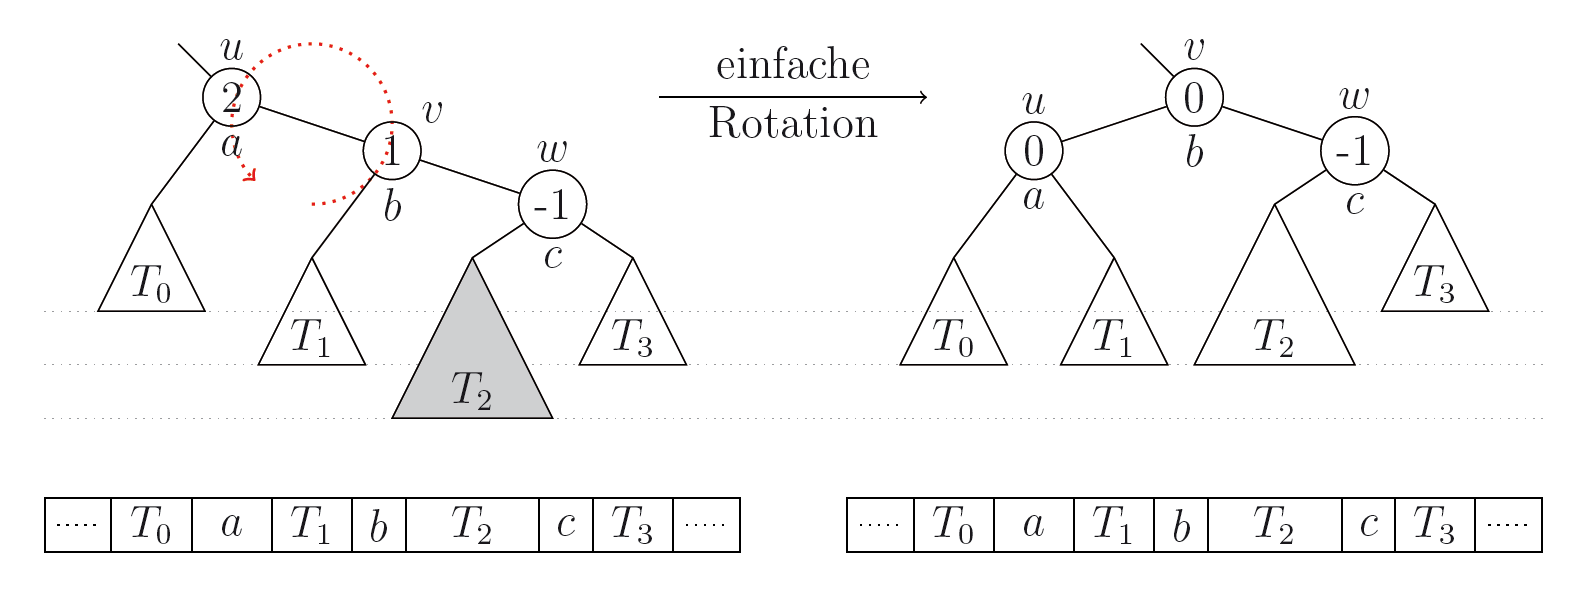
\includegraphics[width=\textwidth]{images/AVL-einfacheRotation.png} \\
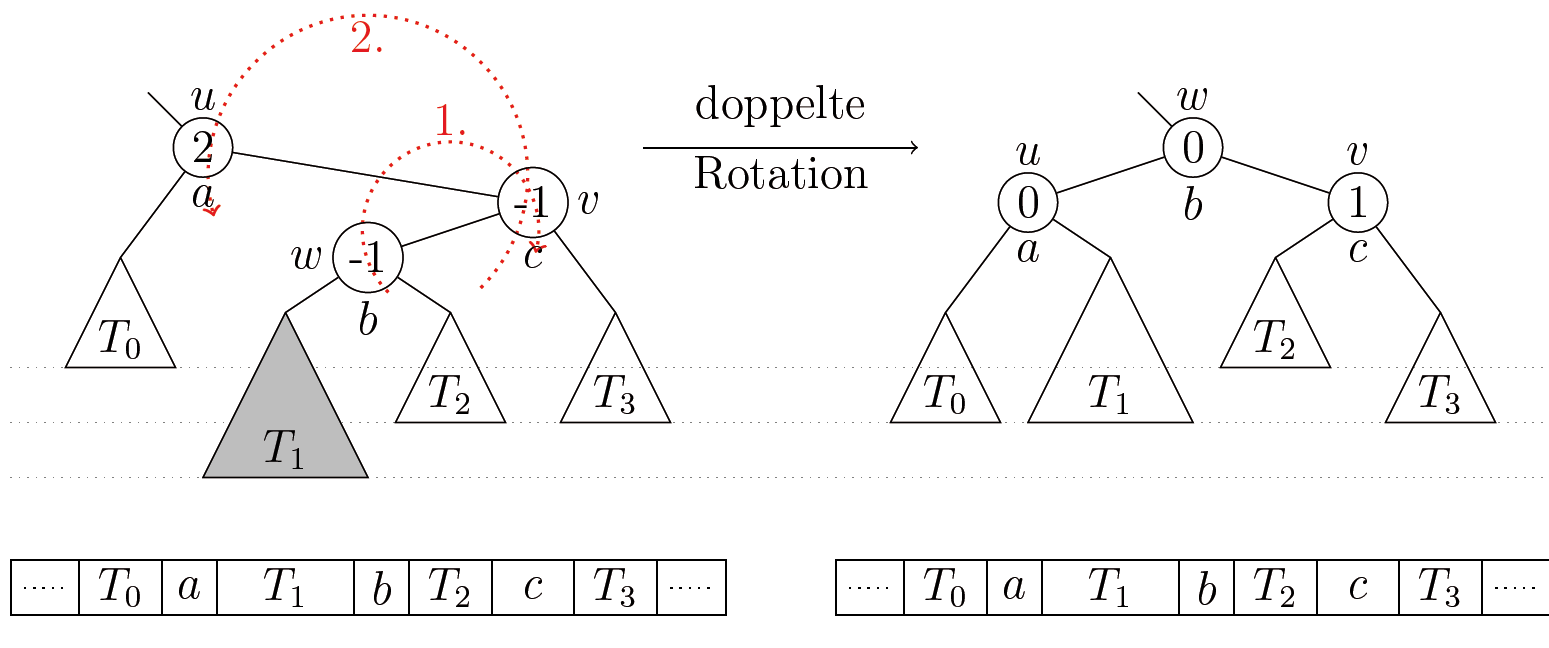
\includegraphics[width=\textwidth]{images/AVL-doppelteRotation.png}

\subsection{Rot-Schwarz-Bäume}
Alternativ kann man bestimmte Knoten von der Eigenschaft für einen perfekten Binärbaum ausnehmen, also "`Färben"':

\begin{shaded}
\begin{tabular}{cc}
schwarz: & normaler Knoten \\
rot: & Ausgleichsknoten (für Höhenunterschiede) \\
\end{tabular}\\
\textbf{Wurzelbedingung:} Die Wurzel ist schwarz. \\
\textbf{Farbbedingung:} Die Kinder von roten Knoten sind schwarze Knoten (oder nil). \\
\textbf{Tiefenbedingung:} Alle Blätter haben die gleiche schwarze Tiefe (definiert als die Anzahl schwarze Vorfahren $-1$) \\ \ \\
Die Höhe eines rot-schwarz Baumes mit $n$ Knoten ist $\Theta(\log n)$
\end{shaded}
Beim Einfügen wird das neue Blatt \rot{rot} (ausser, wenn das neue Blatt die Wurzel ist). Ist der Elternknoten des neuen Blattes jedoch bereits rot, ist die Farbbedingung verletzt. Sollte nach dem Rotieren bei $u$ Doppelrot auftreten, wird solande nach oben iteriert, bis man die Wurzel erreicht.\\
\paragraph{Fall 1: Der Geschwisterknoten $z$ von $v$ ist schwarz:} \ \\
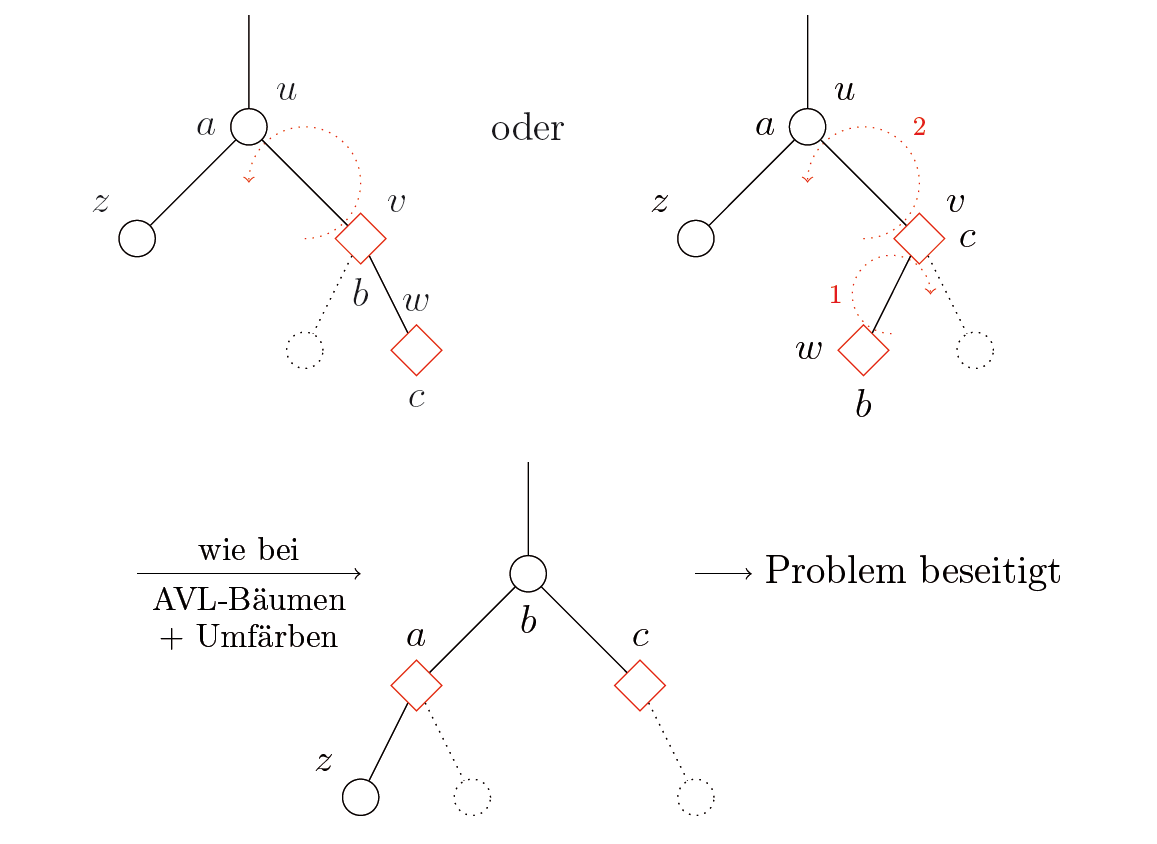
\includegraphics[scale=0.4]{images/RS-Insert1.png}
\paragraph{Fall 1: Der Geschwisterknoten $z$ von $v$ ist rot:} \ \\
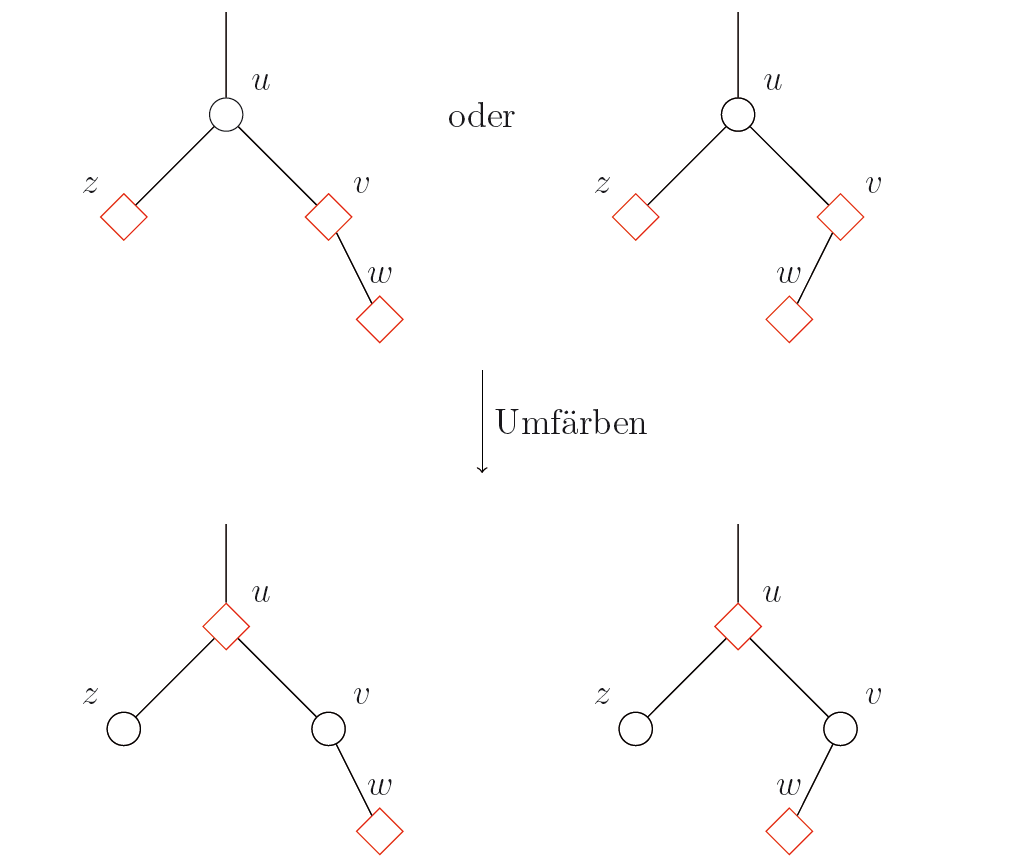
\includegraphics[scale=0.4]{images/RS-Insert2.png}

{\Huge \rot{Löschen von AVL-Bäumen (S.53-55 im Script)}}

\subsection{B-Bäume}
Ist der Index zu groß, müssen Werte evtl weit verstreut abgelegt werden. \\

\begin{shaded}
\underline{Vielwegbaum:} speichert pro Knoten mehrere Schlüssel in aufsteigender Reihenfolge. Zwischen je zwei Schlüsseln, sowie vor dem Ersten und nach dem Letzten wird in Kind/Teilbaum angehängt. Die Zahl der Kinder ist immer Anzahl Schlüssel $-1$

\underline{B-Baum} der Ordnung $d$, $d\geq 2$ \\
\textbf{Wurzelbedingung:} Die Wurzel hat mindestens $2$ und höchstens $d$ Kinder. \\
\textbf{Knotenbedingung:} Jeder andere Knoten hat mindestens $\lceil \frac{d}{2}\rceil$ und höchstens $d$ Kinder. \\
\textbf{Schlüsselbedingung:} Jeder Knoten mit $i$ Kindern hat $i-1$ Schlüssel. \\
\textbf{Tiefenbedingung:} Alle Blätter haben dieselbe Tiefe. \\ \ \\
Ein B-Baum der Ordnung $d$ miz $n$ Knoten hat Höhe $\Theta(\log_d n)$
\end{shaded}

\paragraph{\texttt{insert}:} Suche das Blatt, in das eingefügt werden soll. Wieviele Schlüssel hat das Blatt?
\begin{description}
	\item[$<d-1$] einfügen, fertig
	\item[$=d-1$] Überlauf: teile die $d$ Schlüssel auf in die kleineren $\lfloor \frac{d}{2} \rfloor$ und die größeren $\lceil \frac{d}{2} \rceil+1$, für die zwei neue Knoten erzeugt werden. Das mittlere $(\lfloor \frac{d}{2} \rfloor)$-te wird im Elternknoten eingefügt, evtl Überlauf im Elternknoten durch nach oben iterieren beheben.
\end{description}

\paragraph{\texttt{remove}:} Suche den Knoten, aus dem ein Schlüssel entfernt werden soll. Wieviele Schlüssel enthält er?
\begin{description}
	\item[$>\lceil\frac{d}{2}\rceil -1$] löschen, fertig
	\item[$=\lceil\frac{d}{2}\rceil -1$] Unterlauf
	\begin{enumerate}
		\item Knoten ist innerer Knoten (d.h. kein Blatt)\\
		Ersetze Schlüssel durch Inorder-Vorgänger (oder Nachfolger), d.h. letzten Schlüssel im rechtesten Blatt des vorangeheneden Teilbaumes.
		\item Knoten ist Blatt \\
		Falls ein direkter rechter oder linker Geschwisterknoten mehr als $\lceil\frac{d}{2}\rceil -1$ Schlüssel enthält, verschiebe den Letzten bzw Ersten von dort in den gemeinsamen Vorgänger und den trennenten Schlüssel von vorher in den Knoten mit Unterlauf. \\
		Anderfalls Knoten mit einem der direkten Geschwisterknoten und dem trennenden Schlüssel aus dem Vorgänger verschmelzen.
	\end{enumerate}
\end{description}

%%%%%%%%%%%%%%%%%%%%%%%%%%%%%%%%%%%%%%%%%%%%%%%%%%%%%%%%%%%%%%%%%%%%%%%%%%%%%%%%%%%%%%%%
%%%%%%%%%%%%%%%%%%%%%%%%%%%%%%%%%%%%%%%%%%%%%%%%%%%%%%%%%%%%%%%%%%%%%%%%%%%%%%%%%%%%%%%%
%%%%%%%%%%%%%%%%%%%%%%%%%%%%%%%%%%%%%%%%%%%%%%%%%%%%%%%%%%%%%%%%%%%%%%%%%%%%%%%%%%%%%%%%

\section{Streuen}
Betrachten ungeordnete Wörterbücher. Schlüssel ohne Sortierreihenfolge gespeichert.

\begin{shaded}
\textbf{Bezeichnungen:} \\
\begin{tabular}{ll}
(Schlüssel-)Universum &$\mathcal{U} \subseteq \mathds{N}_0$ \\
Schlüsselmenge & $K \subseteq \mathcal{U}, \; \vert K \vert = n$ \\
Hashtabelle & $H[0,\ldots, m-1]$ (Array von Zeigern) \\
\end{tabular}
\end{shaded}
Eine Hashfunktion $h: \mathcal{U} \to \{0,\ldots,m-1\}$ weisst jedem Schlüssel $k\in\mathcal{U}$ seine Speicherstelle $H[h(k)]$ zu. Im Optimalfall ist jede Stelle in der Hashtabelle nur einfach besetzt ($\Rightarrow$ Einfügen, Suchen, Löschen in $\Theta(1)$). \\
Beispiele für Hashfunktionen:
\begin{itemize}
	\item $h(k) = k \mod m$ \; für Primzahl $m$ (Divisions- /Kongruenzmethode)
	\item $h(k) = \lfloor m\cdot(k\alpha-\lfloor k\alpha\rfloor)\rfloor$, zBsp für $\alpha=\phi^{-1}=\frac{\sqrt{5}-1}{2}\approx 0,61803$ \; (Multiplikationsmethode)
\end{itemize}

\subsection{Kollissionen}
Im Allg. kommt vor: $h(k_1)=h(k_2)$ für einige $h_1,h_2\in K$ $\Rightarrow$ heisst \emph{Kollision}, $k_1,k_2$ heissten \emph{Synonym}.
\begin{shaded}
$p_{m,n} := P \textrm{(keine Kollision)} = 1\cdot\frac{m-1}{m}\cdot\frac{m-1}{m}\cdot\ldots\cdot\frac{m-n+1}{m}$ \\
Schlüssel werden durch $h$ gleichmässig gestreut, d.h. alle Positionen gleich wahrscheinlich. (Bsp. Geburtstagsparadoxon) \\ \vspace{2em}
Erwartete Anzahl Kollisionen: \\
Sei $X_{ij}=
\begin{cases}
1 & \textrm{falls } h(k_i)=h(k_j) \textrm{\tiny (Also bei Kollision)} \\
0 & sonst
\end{cases}$\\
Bei Gleichmässiger Streuung: $E(X)=E\left(\sum_{i<j}X_{ij}\right)=\binom{n}{2}\cdot\frac{1}{m}$ \\
Im Allgemeinen: $E(X)\geq 1 \Leftrightarrow n(n-1)\geq 2m$ \\ \vspace{2em}
\underline{Belegungsfaktor} (load factor): $\beta = \frac{n}{m}$\\
Erwartete Anzahl Leerfelder: $m-m\cdot e^{-\beta} = m(1-e^{-\beta})$
\end{shaded}

\subsection{Kollisionsbehandlung}
\subsubsection{Verkettung}
In der Hashtabelle wird eine Liste von Elementen angelegt. Wenn mehrere Zugriffe auf Zeiger erfolgen, heisst dies \underline{Sondieren}. Im Mittel sind $n=m\ln m$ Einfügungen nötig, um alle Felder zu füllen, dann ist $\beta=\frac{m\ln m}{m}=\ln m > 1$
\subsubsection{Open Hashing}
Idee: In jedem Feld wird nur ein Element gespeichert. $\Rightarrow$ Bei Kollision muss neuer Platz gefunden werden. Wähle dazu eine Folge $d_1,d_2,\ldots,d_i \in \mathds{Z}$ und versuche \[ H[(h(k)+d_i) \mod m], \; i=1,2,\ldots \]
Für $(d_i)$ gibt es verschiedene Wahlen: \\
\begin{tabular}{rp{13cm}}
lineares Sondieren & $d_i=i$ \\
quadratisches Sondieren & $d_i=i^2$ \\
double Hashing & $d_i=i\cdot h'(k)$, wobei $h':\mathcal{U}\to \{1,\ldots,m-1\}$ eine zweite Hashfunktion mit $h'(k) \not= 0 \; \forall k\in\mathcal{U}$ und $m$ prim ist. \\
\end{tabular}

\subsubsection{Kollisionsvermeidung}
Ziel: Gleichmässiges Streuen durch Hash-Funktion\\
Problem: Wissen nicht, welche Schlüssel gespeichert werden sollen. \\
Idee: Wähle aus einer Menge von Hashfunktionen $\mathcal{H} \subseteq \{h:\mathcal{U} \to \{0,\ldots,m-1\}\}$ zufällig eine aus.
\begin{shaded}
Eine Familie von Streufunktionen heisst \underline{universell}, falls \[ \vert \{h\in\mathcal{H}: h(k_1) = h(k_2)\}\vert \leq \frac{\vert \mathcal{H}\vert}{m}\;\forall k_1,k_2\in\mathcal{U} \]
\end{shaded}
Bei zufälliger Wahl sind wir berechtigt $P(h(k_1)=h(k_2))=\frac{1}{m}$ anzunehmen. \\

\rot{Das ist mir jetzt grad zu blöd die Formeln weiter abzutippen, Seite 68ff}

\subsubsection{Bloom-Filter {\tiny (aus der Übung)}}
Bloom-Filter besteht aus $m$ Bits, die zu Beginn 0 sind, $k$ verschiedenen Hash-Funktionen mit Wertebereich $\{0,\ldots,m-1\}$ \\
\begin{description}
	\item[Einfügen:] Berechne alle $k$ Hashwerte und setze die entsprechenden Bits auf 1.
	\item[Suchen ob drin:] Berechne $k$ Hashwerte
	\begin{itemize}
		\item wenn alle Bits $0$, auf keinen Fall enthalten
		\item wenn alle Bits $1$, mit sehr großer Wahrscheinlichkeit enthalten
		\item wenn einige Bits $1$, evtl vorhanden
	\end{itemize}

\end{description}

%%%%%%%%%%%%%%%%%%%%%%%%%%%%%%%%%%%%%%%%%%%%%%%%%%%%%%%%%%%%%%%%%%%%%%%%%%%%%%%%%%%%%%%%
%%%%%%%%%%%%%%%%%%%%%%%%%%%%%%%%%%%%%%%%%%%%%%%%%%%%%%%%%%%%%%%%%%%%%%%%%%%%%%%%%%%%%%%%
%%%%%%%%%%%%%%%%%%%%%%%%%%%%%%%%%%%%%%%%%%%%%%%%%%%%%%%%%%%%%%%%%%%%%%%%%%%%%%%%%%%%%%%%

\section{Dynamische Programmierung: Ausrichten}
Idee: Suchen nach "`ähnlichen"' Wortketten.
\begin{shaded}
\begin{itemize}
	\item $\Sigma$ ist Alphabet
	\item $s=a_1a_2\cdots a_n\in\Sigma^*=\bigcup \Sigma^k$ heisst "`Wort"' oder "`Sequenz"' der Länge $\vert s\vert=n$
	\item $\varepsilon$ ist das leere Wort, $\vert\varepsilon\vert=0$
	\item Teilsequenz $s'$ von $s=s=a_1a_2\cdots a_n$ erfüllt $s'=a_i\cdots a_j$ für $1\leq i,j\leq n$ (im Unterschied zum Teilwort, bei dem auch Zeichen ausgelassen werden können.
\end{itemize}
\vspace{2em}
Um zwei Wörter zu vergleichen, gibt es drei Operationen. Ähnlichkeit ist die minimale Anzahl Operationen
\begin{description}
	\item[Substitution:] Ein Zeichen wird durch ein anderes ersetzt.
	\item[Einfügung:] Ein Zeichen wird in einem Wort hinzugefügt.
	\item[Löschung:] Ein Zeichen wird in einem Wort entfernt
\end{description}
\vspace{2em}

Ein Paar heisst $\overline{s},\overline{t}\in\Sigma^*\times\Sigma^*$ \underline{Ausrichtung} von $s,t\in\Sigma^*$, falls
\begin{itemize}
	\item $\overline{s}\vert_\Sigma=s,\overline{t}\vert_\Sigma$ {\tiny (Weglassen aller Leerzeichen ergibt Ausganssequenz)}
	\item $\vert\overline{s}\vert=\vert\overline{t}\vert$ {\tiny (Beide Sperrungen gleich lang)}
	\item \rot{Bewertung und Editierbarkeit Script S74}
\end{itemize}
\vspace{2em}
\end{shaded}

\rot{Der Ausrichtalgorithmus aus der Übung} \\

Eine optimale Ausrichtung kann in $\mathcal{O}(nm)$ mit $\mathcal{O}(\min\{n,m\})$ Platz bestimmt werden.

%%%%%%%%%%%%%%%%%%%%%%%%%%%%%%%%%%%%%%%%%%%%%%%%%%%%%%%%%%%%%%%%%%%%%%%%%%%%%%%%%%%%%%%%
%%%%%%%%%%%%%%%%%%%%%%%%%%%%%%%%%%%%%%%%%%%%%%%%%%%%%%%%%%%%%%%%%%%%%%%%%%%%%%%%%%%%%%%%
%%%%%%%%%%%%%%%%%%%%%%%%%%%%%%%%%%%%%%%%%%%%%%%%%%%%%%%%%%%%%%%%%%%%%%%%%%%%%%%%%%%%%%%%

\section{Graphen}
\subsection{Definitionen}
\begin{shaded}
Das Paar $G=(V,E)$ aus den Mengen $V$ und $E\subseteq\binom{V}{2}$ heisst (endlicher, ungerichteter) Graph, Elemente aus $V$ heissen Knoten, Elemente aus $E$ heissen Kannten. Allgemein: $n=n(G)=\vert V\vert$ und $m=m(g)=\vert E\vert$. \\
Zwei Knoten $u,v\in V$ heissen \underline{adjazent} (benachbart), falls es eine Kante $\{u,v\}\in E$ gibt. \\
Die \underline{Adjazenzmatrix} $A(G)=(a_{v,w\in V}$ mit \[a_{v,w}=
\begin{cases}
1 & \textrm{falls } \{v,w\} \in E \\
0 & \textrm sonst
\end{cases} \] \\
Die \underline{Inzidenzmatrix} $I(G)=(i_{v,e})_{v\in V \wedge e\in E}$ mit \[i_{v,e}=
\begin{cases}
1 & \textrm{falls } v\in e \\
0 & \textrm sonst
\end{cases} \] \\
Ein Knoten $v\in V$ und eine Kante $e\in E$ heissen \underline{inzident}, falls $v\in e$. \\
Die Menge der zu $v$ adjazenten Knoten heisst \underline{Nachbarschaft} und deren Kardinalität \underline{Grad} $d_G$\\
Ein \underline{Teilgraph} $G'=(V',E')$ mit $V'\subseteq V, E'\subseteq E$ heisst \underline{Teilgraph} von $G$, $G$ \underline{enthält} $G'$.\\
Ein Teilgraph heisst \underline{aufspannend}, wenn er alle Knoten enthält.\\
Gibt es zu zwei Graphen $G_1,G_2$ eine isomorphe Abbildung, so heissen $G_1$ und $G_2$ \underline{isomorph} \\
Ein $(s,t)$-\underline{Weg} der Länge $k$ ist vorhanden, wenn eine Verbindung mit $k$-Kanten zwischen $s$ und $t$ besteht. Der kürzeste Weg heisst \underline{Abstand} oder \underline{Distanz}. \\
Ein \underline{Kreis} ist ein Weg, der denselben Start- wie Endknoten hat. \\
Ein Graph heisst \underline{zusammenhängend}, wenn es zu je zwei Knoten $s,t\in V$ einen Weg gibt. ($\Rightarrow$ Zusammenhangskomponenten)\\
\vspace{2em}
Für alle Graphen $G=(V,E)$ gilt: $\displaystyle\sum_{v\in V}d_G(v)=2m$. Die Anzahl der Knoten ungeraden Grades ist gerade. Es gibt immer zwei Knoten mit gleichem Grad.
\end{shaded}

\subsection{Bäume und Wälder}
\begin{shaded}
Ein zusammenhängender Graph ohne Kreis heisst \underline{Baum}. Ein Graph, dessen Zusammenhangskomponenten Bäume sind, ist ein \underline{Wald}. \\
Für jeden Graphen $G=(V,E)$ gilt: $m\geq n-\kappa(G)$, Bei Gleichheit ist $G$ ein Wald.\\ \vspace{2em}
Für einen Graphen sind folgende Aussagen äquivalent:
\begin{enumerate}
	\item $G$ ist ein Baum.
	\item Zwischen je zwei Knoten in $G$ existiert genau ein Weg.
	\item $G$ ist zusammenhängend und hat $n-1$ Kanten.
	\item $G$ ist minimal zusammenhängend.
	\item $G$ ist maximal kreisfrei.
\end{enumerate}
Jeder zusammenhängende Graph enthält einen Baum. Die Anzahl $\mu(G)=m-n+\kappa(G)$ heisst \underline{zyklomatische Zahl}. \\
\rot{Kanzenzugdefinitionen usw S86} \\
Eine Tour heisst \underline{Eulertour} falls sie jede Kante genau einmal enthält. Ein Graph enthält genau dann eine Eulertour, wenn alle Kanten geraden grad haben.
\end{shaded}

\subsection{Tiefensuche}
Idee: Knotenstack speichert noch zu bearbeitende Knoten. Wir gehen zuerst über Nachbarn in die Tiefe, wenn keine Knoten mehr vorhanden sind, gehen wir zum letzten bereits besuchten Knoten zurück, der noch unbesuchte Nachbarn hat.
\subsubsection{Laufzeit}
Die Laufzeit ist in $\mathcal{O}(n+m)$

\subsection{Breitensuche}
Idee: Knotenwarteschlange (Queue), wir besuchen von einem Knoten erst alle Nachbarn. Jeder markierte Knoten wird in die Queue gelegt. Dann wird jeweils der vorderste entnommen und von diesem alle Nachbarn besucht.
\subsubsection{Laufzeit}
Die Laufzeit ist in $\mathcal{O}(n+m)$

\subsection{Kürzeste Wege}
Betrachten nun gerichtete Graphen. Kanten werden durch Gewichte unterschiedlich bewertet (labeled). \\
\begin{shaded}
\textbf{Single-Source Shortes-Path} Problem {\tiny (SSSP)}:\\
geg: gerichteter Graph $G=(V,E,\lambda)$ mit Kantenlängen/-gewichten $\lambda:E\to\mathds{R}$\\
ges: Kürzeste Wege zu allen Knoten
\end{shaded}

\subsubsection{Algorithmus von \textbf{Dijkstra}}
Idee: Wir optimieren lokal und hangeln uns dann im Graph weiter vor.\\
Dazu wird jeweils der aktuell kürzeste Pfad zu jedem Knoten gespeichert. Wenn ein Knoten noch nicht besuchte inzidente Kanten hat, wird er in eine Warteschlange gelegt. Für den vordersten Knoten in der Warteschlange wird nun überprüft, welche inzidente Kante den kürzesten Weg zum nächsten Knoten bildet, dieser wird mit dem aktuell kürzesten Weg zum gerade Betrachteten Knoten addiert und dem neuen Knoten gutgeschrieben. Wenn der neuen Knoten bereits einen Weg hat, wird der kürzere der beiden genommen.\\ Einschränkung: funktioniert nur mit nicht-negativen Kantengewichten.
\paragraph{Laufzeit} Je nach verwendeter Struktur zur Speicherung des Graphen bis zu $\mathcal{O}(m+n\log n)$ {\tiny Fibonacci-Heap} bzw $\mathcal{O}(n+m\log n)$ {\tiny Heap aus Kapitel 2}

\subsubsection{Algorithmus von \textbf{Bellman/Ford}}
Vorteil: Kann auch mit negativen Kantengewichten umgehen.\\
Nachteil: Benötigt $\mathcal{O}(nm)$ \\
Nicht möglich bei: enthaltene Zykel negativer Länge {\tiny sonst würde er unendlich diesen Zykel nehmen...} \\
Führt Relaxationen in schematisch fester Reihenfolge durch.

%%%%%%%%%%%%%%%%%%%%%%%%%%%%%%%%%%%%%%%%%%%%%%%%%%%%%%%%%%%%%%%%%%%%%%%%%%%%%%%%%%%%%%%%
%%%%%%%%%%%%%%%%%%%%%%%%%%%%%%%%%%%%%%%%%%%%%%%%%%%%%%%%%%%%%%%%%%%%%%%%%%%%%%%%%%%%%%%%
%%%%%%%%%%%%%%%%%%%%%%%%%%%%%%%%%%%%%%%%%%%%%%%%%%%%%%%%%%%%%%%%%%%%%%%%%%%%%%%%%%%%%%%%

\section{amortisierte Analyse}
Idee: wir wollen eine schärfere Laufzeitschranke finden, als wir dies normal könnten. Verwenden dazu die "`Bank-Account-Method"', betrachten die Gesamtlaufzeit, nicht die einzelnen Operationen. Werden bei zeitlich früherer Operation mehr "`Zeit verbuchen"' als nötig, um dadurch folgende Operationen günstiger zu bekommen.
\subsection{Beispiel: Binärzähler}
Kosten: $\left.
\begin{tabular}{c|c}
	 & reale Kosten \\
	\hline
	0 & \\
	1 & 1 \\
	10 & 2 \\
	11 & 1 \\
	100 & 3 \\
	101 & 1
\end{tabular} \right\rbrace \Rightarrow$ sehr unterschiedliche Kosten \\
\vspace*{2ex} \\
\begin{tabular}{|c|c|c|c|c}
\hline
   &   &   & 5 & $\curvearrowright 1 \curvearrowright 10$ \\
\hline
   &   & 5 & 4 & $\curvearrowright 11$ \\
\hline
   &   & 5 & 8 & $\curvearrowright 100$ \\
\hline
   & 5 & 4 & 7 & $\curvearrowright 101$ \\
\hline
   & 5 & 4 & 11 & $\curvearrowright 111$ \\
\hline
   & 5 & 8 & 15 & \\
\hline
\end{tabular}
\\ \vspace{2ex} \\
\begin{tabular}{c|c|c}
 & normale Analyse & amortisierte Analyse \\
eine Einfügeoperation & $\mathcal O(\log n)$ & \\
$n$ Operationen & $\mathcal O(n\log n)$ & $\mathcal O(n)$
\end{tabular}

\end{document}
